\documentclass[a4paper, 12pt]{article}

\usepackage{fancyhdr}
\pagestyle{fancy}
\lhead{PROJET : Forteresse}
\lfoot{Info Sup}
\rfoot{EPITA 2016}
\renewcommand{\footrulewidth}{0.3mm}

\usepackage[french]{babel}
\usepackage{listings}
\usepackage[T1]{fontenc}
\usepackage{eurosym}
\usepackage{setspace}
\usepackage{caption}

\usepackage[utf8]{inputenc}
\usepackage{graphicx}

\renewcommand{\baselinestretch}{1.5}
\begin{document}
\begin{titlepage}
  \begin{sffamily}
  \begin{center}

    % Upper part of the page. The '~' is needed because \\
    % only works if a paragraph has started.

    \textsc{\Huge Rapport soutenance 2}\\[3cm]

    \textsc{\LARGE Projet:}\\[1.5cm]

    % Title
	\centerline{\includegraphics{coollogo_com-19602433.png}}
	\vfill{
	\centerline{\includegraphics[scale=0.4]{crossed-swords-clip-art-48219.jpg}}}

    % Author and supervisor
    \begin{minipage}{0.4\textwidth}
      \begin{flushleft} \large	
      
      \end{flushleft}
    \end{minipage}
	\begin{flushleft}\vfill
      {
       \textsc{Chatelus} Florian - \emph{chatel\_f} \\
       \textsc{Henric} Arnaud - \emph{henric\_a}\\
       \textsc{Sarkar} Riday - \emph{sarkar\_r}\\
       }
    \end{flushleft}	
  \end{center}
  \end{sffamily}
\end{titlepage}

\begin{spacing}{1.0}
	\tableofcontents
\end{spacing}

\newpage
\section{Introduction}
Dans le cadre de de notre première année à l'EPITA, nous devons réaliser un projet informatique de fin d'année qui doit montrer l'application de nos connaissances dans le domaine de la programmation.
Le sujet étant libre, nous avons décidé de réaliser un jeu vidéo nommé Forteresse.
Le présent document est  le rapport de la première soutenance qui retrace l'avancement de notre projet en cours de développement depuis la validation du cahier des charges jusqu'à la première soutenance. Ainsi, à travers ce rapport, nous allons établir un bilan des tâches qui ont été réalisées par chacun des membres du groupe. Nous allons aussi établir un bilan  des tâches qui restent à  réaliser pour  la prochaine soutenance.

\newpage

\section{Présentation}
	\subsection{Les membres du groupe}
	\parindent=0cm\textbf{Florian \textsc{Chatelus}}
	\smallbreak
	\par \parindent=0.5cm Commence enfin l'une des raisons pour laquelle j'ai choisi l'EPITA, le projet! A mon arrivé a l'EPITA la programmation ne m'était pas totalement inconnue puisque j'ai eu la chance de pouvoir choisir la spécialisation ISN en Terminale. Nous avions réussi avec mon groupe a recréer le célèbre PONG. Bien que mon projet d'ISN ai été très basique, je pense qu'il me servira au moins dans les démarches de réalisation du projet. J'ai donc une petite expérience en ce qui concerne le travail de groupe, que j'espère arriver a mettre a profit pour notre projet de cette année. Malgré tout, ce projet sera un réel challenge pour moi, puisqu'il nous obligera a faire appel a de nombreuse compétence que nous ne disposons pas encore. Ce sera donc un formidable exercice, qui demandera une certaine rigueur dans le travail certes, mais qui me permettra de progresser rapidement.\\
	
	\parindent=0cm\textbf{Arnaud \textsc{Henric}}
	\smallbreak
	Le projet de première année, enfin ! Nous avons déjà eu des TPs de programmation mais le projet permettra de nous tester d’avantage. En groupe, nous allons réaliser un devoir que nous avons nous-mêmes choisi, un jeu-vidéo. J’ai déjà réaliser certains projets en ISN au lycée (le triangle de Sierpinski, le jeu de la vie ou encore un code barre) mais jamais de projet comme celui-ci, sur un semestre entier et en groupe. Néanmoins ISN m’a donné un peu d'expérience et je suis prêt à créer ce jeu vidéo.\\
\newpage	
	\parindent=0cm\textbf{Riday \textsc{Sarkar}}
	\smallbreak
 Avant d’arriver à EPITA,  j'ai jamais touché à une ligne de code à part cliquer de temps en temps sur des icônes avec Algobox en cours de maths (au passage c'était très bien pour découvrir  le monde merveilleux de l’algorithmique). Je suis conscient que réaliser les tâches qu’on m’a données ne sera pas facile. Cela étant dit, je sais que ce projet est un plus pour nous et qu’on va apprendre beaucoup de choses à travers la réalisation de ce projet. Donc je vais jouer le jeu et faire un maximum de choses pour le projet et essayer d’apprendre un maximum de choses à travers la réalisation de ce projet.\\

	\parindent=0.5cm 
	\subsection{Les origines du projet}
Nous avons choisi de réaliser un jeu plutôt qu’un logiciel car nous avons deux membres dans le groupe qui ont déjà réalisé un jeu en Terminale dans le cadre d’un projet en groupe. Même si le projet achevé en ISN par ces deux derniers n’est pas comparable avec ce qui nous attend ce semestre en INFO SUP, ce sera toujours une aide non-négligeable.
\par Une fois que la nature du projet était choisi, nous avons réfléchi longuement sur le type de jeu que nous allons réaliser. Notre expérience en tant que joueur nous donnait un large choix parmi les types de jeu possibles comme un RPG (Role Playing Game), RTS (Real Time Strategy) ou encore un Tower Defense . 

	\subsection{Le jeu}
		\subsubsection{Présentation}
		\par Notre jeu sera basé sur le principe du \textit{tower defense}. Qu'est-ce que 			cela signifie? Un \textit{tower defense}, est un jeu qui comme son nom l'indique 			aura comme objectif de défendre un point donné. Le but du jeu sera donc de défendre 		un cristal qui alimente la porte de l'endroit que nous souhaitons protéger.  
		\subsubsection{Déroulement d'une partie}
		Une partie se déroulera en deux phases qui se répéteront, a chaque vague d'ennemis.\\
		\centerline{\includegraphics[scale=0.55]{Plan.png}}
		\par La première est la phase que nous appellerons \textit{phase de préparation}, elle consiste à préparer ses défenses, en les positionnant de façon stratégique, les améliorant ou en les réparant. Cette phase sera d'une importance capital pour assurer une victoire lors de la phase suivante. Une fois que vous serez fin prêt pour le combat, il vous suffira d'appuyer sur prêt et la deuxième phase commencera une fois tout les joueurs prêt.
		\par Nous arrivons donc en deuxième phase, la \textit{phase de combat}, qui va déclencher l'action. Des créatures vont apparaitre à des points précis de la carte et vont converger vers le ou les cristaux. Le joueur pourra donc durant cette phase attaquer les monstres et tenter de les détruire et/ou continuer à poser, améliorer et réparer ses constructions mais avec des malus d'incantation.
		\bigbreak
		\begin{figure}[!ht]
			\centerline{\includegraphics[scale=0.3]{cristalprojet.png}}
			\caption*{Image du cristal à protéger}
		\end{figure}
		\par Tous les certains nombre de cycle, au terme de ces deux phases, un monstre plus imposant apparaitra, et le joueur devra s'en défaire afin de remporter la manque et d'obtenir des objets.
		\subsubsection{Multijoueur}
		Le mode multijoueur consistera en un mode CO-OP. Vous devrez \^etre capable de jouer en \'equipe afin d'affronter vos adversaires. Pour cela, vous commencerez la partie c\^ote \'a c\^ote. Vous ne pouvez combattre seulement des IA. Le mode multijoueur consiste en un mode en \'equipe et non pas en 1vs1 contre un ami.
		\par Chaque joueur pourra int\'eragir avec l'environnement. Leurs constructions et leurs objectifs sont communs tandis que toutes leurs caract\'eristiques telles que leur monnaie et leur vie sont s\'epar\'ees.
		\subsubsection{L'interface}
		L’interface permettra au joueur d'être renseignée à tout moment sur : 
		\begin{itemize}
		\item Le temps écoulé.
		\item Sa jauge de vie.
		\item L’arme dont il est en possession , ainsi que les  munitions dont il dispose.
		\item L’argent qu’il possède pour acheter de nouvelles tours ou armes.
		\end{itemize}
		\subsubsection{L'arsenal de défense}
		Nous utiliserons donc différents types d’armes de type médiéval fantastique.
Les armes seront donc accessible en la ramassant sur un bosse ou bien  suite à un achat du joueur, elles pourront être améliorer, durant la partie. On distinguera plusieurs types d’armes tel que:
	\begin{itemize}
	\item Les épées.
	\item Les arcs.
	\item Les bâtons.
	\end{itemize}
Les défenses fixes seront achetable grâce a l’argent gagné durant la partie. Les défenses seront comme les armes améliorables. Ces dernières seront autonomes et feront partie de l’IA. On pourra y trouver:
	\begin{itemize}
	\item Des tourelles.
	\item Des pièges.
	\item Des auras.
	\end{itemize}
\newpage
\section{Répartition des tâches}
Nous avions au départ attribué deux personnes a chaque tâche, afin de pouvoir nous entre aider. cela nous a servit puisqu'un membre du groupe nous a quitté, toute les tâches ont donc gardé au moins une personne attribué. Mais il s'est avéré plus efficace de se spécialiser dans des domaines précis plutôt que de toucher a beaucoup de domaine et de travailler a plusieurs sur ceux-ci.\\
Le tableau ci dessous montre quelles ont été les tâches effectué et par qui.
\bigbreak
\bigbreak
	\begin{tabular}{|c||c|c|c|c|c|}
		\hline
		& Florian & Riday & Arnaud \\
		\hline
		Site & & & $\times$\\
		\hline
		3D & & &\\
		\hline
		2D & & & \\
		\hline
		IA & $\times$ & & \\
		\hline
		Multijoueur &  & &\\
		\hline
		Réseau & & & \\
		\hline
		Menu & & & $\times$\\
		\hline
		Gameplay & $\times$ & &\\
		\hline
		Animation & $\times$ & & \\		
		\hline
		Audio & & & $\times$\\
		\hline
		\LaTeX & $\times$ & $\times$ & $\times$\\
		\hline
	\end{tabular}
	\newpage
\newpage
\section{Avancement du projet}
	\subsection{Le graphisme}
		\subsubsection{La carte}
		Notre but pour la deuxième soutenance était de finir la première carte et de commencer la deuxième. Lors de la première soutenance, nous avions une première carte qui n'était pas riche en détail. Pour commencer, il faillait donc rendre riche en détail cette première carte. Pour cela, nous avons décidé d’ajouter des villages dans la carte. Nous nous sommes renseignés concernant les villages médiévaux et nous avons essayer de construire des villages de façon à ce qu’ils ressemblent au mieux aux villages de l'époque médiévale.    
\par Nous avions décidé de différencier la deuxième carte de la première. Dans la première carte, nous avons un terrain plutôt vert avec des chaînes de montagnes qui l’entourent, des arbres et des maisons qu’on pouvait trouver dans des villages de l'époque médiévale. Nous avons donc décidé de changer de décor dans la deuxième carte et d’avoir un environnement plutôt  urbain. Dans la deuxième carte, nous avons toujours une carte fermée. Mais au lieu des montagnes, nous avons entouré le terrain par des murs avec une texture de brick pour avoir une environnement urbain. Nous avons aussi modifié les villages en commençant par les types de maisons, les autres éléments constituant d’un village et leurs disposition.


		\subsubsection{La 3D}
		Notre but pour cette deuxième soutenance était d’avoir plusieurs modèles de personnages ainsi que plusieurs modèles d’ennemis. Pour le moment, nous avons deux modèles de personnages et trois modèles d’ennemis. Ainsi avant de lancer la partie, le joueur a la possibilité de choisir un modèle de personnages parmi les deux. Comme nous l’avons déjà dit lors de la première soutenance, nous avons décidé de ne pas passer du temps à modéliser les personnages mais de les prendre de l’asset store. Mais nous sommes limités dans nos choix puisqu’il n’y a pas beaucoup de modèles de personnages disponible sur l’asset store qui vont avec l’époque médiévale.  Pour construire les villages dans les deux cartes, nous avons des modèles de maisons et tous les éléments constituant d’un villages comme les fontaine par exemple.


		\subsubsection{La 2D}
Lors de la première soutenance, nous avions deux barre de vie qui n'étaient pas fonctionnelles et nous avions pas de véritable interface de jeu. Notre but pour la deuxième soutenance était de faire fonctionner les barres de vie ainsi de commencer d’avoir une interface de jeu. 
\par Nous avons deux barres de vie différentes parmi les quelles nous avons une barre qui est destinée pour la vie du joueur et une autre pour la vie du cristal. Pour différencier ces deux barres de vie, nous avons ajouté une image du cristal devant la barre de vie du cristal et une image d’un guerrier médiéval devant la barre de vie du joueur.  
\par Le joueur dispose une somme d’argent initiale ainsi il peut construire des tours pour attaquer les ennemis et donc défendre le cristal. Lorsqu’il tue un ennemi en attaquant lui-même ou par l'intermédiaire des tours, il gagne des lingots d’or. Nous avons un affichage qui comptabilise ses gains et ses dépenses. Ainsi il peut donc voir a chaque moment l’argent dont il dispose. Il peut aussi voir les différents différents outils qui sont à sa disposition pour défendre le cristal  c'est-à-dire les différentes tours qu’il peut construire. Le joueur peut aussi voir combien coûte la tour et la touche qu’il faut appuyer pour construire la tour.   
Pour rendre joli cet interface du jeu, nous avons travaillé avec essentiellement deux logiciels du traitement d’image : Paint et GIMP.
	\begin{figure}[!ht]
		\centerline{\includegraphics[scale=0.3]{GUI.png}}
		\caption*{HUD}
	\end{figure}
\par Nous avons aussi mis en place un texte d’introduction qui apparaît lorsqu’on commence une partie. Ce texte explique ce que doit faire le joueur pour commencer le jeu. Puis le texte disparaît lorsque le joueur appuie sur la touche B du clavier.   
L'état actuel du graphisme est avancé.
\subsubsection*{Ce qui est à faire pour la prochaine soutenance}
\begin{itemize}
\item Finir la deuxième carte

\end{itemize}

\newpage

	\subsection{Le réseau}
Nous sommes en retards dans la partie réseau. Lors de la première soutenance, nous avions reporté la partie réseau pour la deuxième soutenance. Pour le moment, nous avons réussi a avoir plusieurs personnages dans la même carte. 



\begin{figure}[!ht]
	\centerline{\includegraphics[scale=0.3]{Menureseauprojet.png}}
	\caption*{Image du menu pour jouer en réseau}
\end{figure}


\subsubsection*{Ce qui est à faire pour la prochaine soutenance}

\par Certes nous avons mis en place le réseau, mais pour l’instant, le joueur qui se comporte comme serveur peut commencer une partie sans qu’il y ait d’autres joueurs présents en ligne. Donc il faut recoder le network manager  pour que joueur qui va se comporter comme serveur ne puisse pas lancer la partie tant qu’il n'y ait pas au moins un autre joueur en ligne.

\newpage
	\subsection{Multijoueur}
	Nous sommes en retards dans la partie multijoueur. Lors de la première soutenance, nous avions reporté la partie multijoueur pour la deuxième soutenance. Mais étant donne que la partie réseau n’est malheureusement  pas pleinement opérationnelle, nous n’avons pas commencé la partie multijoueur. 

	
	\subsection{L'intelligence artificiel}
	Lors de la soutenance 1, les monstres pouvaient uniquement suivre un chemin en boucle et mourir, ils ne remplissaient donc absolument pas leur rôle. L’objectif fixé pour cette soutenance fut donc de les rendre fonctionnels. Les ennemis arrêtes désormais de tourner en boucle dans leurs chemin prédéterminé, ils vont jusqu’à leur dernier « check point » et s’arrêtent. Jusqu’ici il n’y avait aucune interaction avec le joueur, le monstre se contentais d’avancer, il peut désormais détecter lorsqu’un ennemis ou un cristal se trouve proche de lui et va donc se diriger dans sa direction. Le monstre va suivre le joueur a moins qu’il ne s’éloigne assez du monstre, auquel cas il le monstre repartira sur le chemin qui lui est destiné. Lorsqu’il est a porté, il peut désormais attaquer, que ce soit le joueur ou bien le cristal. Il attaquera de façon périodique, les joueurs/cristaux qui se situe devant lui.

	
\subsubsection*{Ce qui est à faire pour la prochaine soutenance}	
	
	\begin{itemize}
	\item une attaque a distance
	\end{itemize}


	\subsection{Le menu}
	
	Le menu se décompose en plusieurs parties. Il concerne le menu principal (où l’on peut lancer le jeu en mode solo, ou bien multijoueur, mais également accéder à un sous-menu d’options ou enfin, quitter le jeu). Ensuite, nous avons un menu de sélection de la carte dans laquelle nous souhaitons jouer, il suffit d’appuyer sur la flèche pour sélectionner une autre carte et d’appuyer sur “play” pour lancer la partie. 
	\begin{figure}[!ht]
		\centerline{\includegraphics[scale=0.3]{choixdemap.png}}
		\caption*{menu du choix de la carte}
	\end{figure}
	\par Enfin, dans une partie, on peut faire une pause et afficher un menu qui arrête momentanément le déplacement des ennemis. Lorsqu’on appuie sur le bouton pour reprendre, la partie et les déplacements des personnages fonctionnent à nouveau normalement. On peut également, dans ce menu, recharger la partie ou encore, revenir au menu principal. Enfin, pour cette soutenance nous avons également ajouté un menu pour sélectionner le héros avec lequel nous souhaitons jouer dans la prochaine partie.

\newpage
	\begin{figure}[!ht]
		\centerline{\includegraphics[scale=0.3]{mainMenu.png}}
		\caption*{Image du menu principal}		
	\end{figure}
	\begin{figure}[!ht]
		\centerline{\includegraphics[scale=0.3]{pauseMenu.png}}
		\caption*{Image du menu pause}
	\end{figure}
	
	\par Enfin, nous avons également créer un menu-pause qui apparaît lorsqu’on appuie sur “echap” dans le jeu. Il arrête bien sûr le jeu (les mouvements des personnages et les attaques) lorsqu’il est actif. Dans le menu pause, on peut évidemment reprendre le jeu en cours au même moment, mais également relancer le niveau et revenir au menu principal. On pourra ensuite sauvegarder le jeu, pour le reprendre plus tard.

	\subsection{Le site}
	 
	\begin{figure}[!ht]
		\centerline{\includegraphics[scale=0.3]{siteprojet.png}}
		\caption*{Page d'accueil du site internet}
	\end{figure}	 
	 
	 Le site internet permet d’avoir une présentation générale du jeu Forteresse. Il permet d’en savoir plus sur les règles du jeu mais on peut aussi avoir un aperçu du gameplay avec différentes images tirées du jeu. Ensuite, on peut suivre les avancées de la réalisation de Forteresse. Sur un autre onglet, on peut également télécharger le jeu en version normale ou encore version lite pour éviter les bandes-annonces et quelques animations. On peut avoir accès au cahier des charges du groupe FAR. Enfin, une dernière page sera configurée pour permettre aux utilisateurs de rentrer en contact avec le groupe pour poser des questions.


	\subsection{Gameplay}
		
		\subsubsection{L'arsenal défensif}
		Tout d’abord afin d’améliorer le gameplay et de le diversifier nous avons décidé d’ajouter un nouvel élément dans notre arsenal de défense. Un sol de braise, il s’utilise de façon différente d’une tour classique, il peut être posé à n’importe quel endroit sur la carte et fait des dégâts aux ennemis lorsque ceux-ci sont sur la partie du sol avec les braises. Cette arme est à privilégier lorsqu’il y a une multitude d’ennemis disposant de peu de point de vie.

	\begin{figure}[!ht]
		\centerline{\includegraphics[scale=0.3]{lavafloor.png}}
		\caption*{sol de braise}
	\end{figure}		
		\subsubsection{Le système d’argent}
		Aspect essentiel de la plupart des jeux, le système de monnaie du jeu est simple, il faut tuer des ennemis pour récupérer l’or qu’ils laissent tomber lors de leur mort. Il existe deux type d’objet a ramasser, les pièces d’or dont la valeur vaut 1 et les lingot d’or dont la valeur vaut 5. Chaque élément de l’arsenal possède un prix nécessaire à sa construction.
	\begin{figure}[!ht]	
		\centerline{\includegraphics[scale=0.3]{gold.png}}	
		\caption*{pièces d'or à ramasser sur le sol}	
	\end{figure}
		
		\subsubsection{L’attaque des personnages}
	
		L’une des particularités de notre Tower Défense est de posséder un personnage pouvant évoluer sur la carte. Mais ce personnage ne se limite pas seulement à poser des tours il est aussi capable de d’attaquer pour combattre les ennemis qui menace le cristal. Le guerrier est doté d’une attaque au corps à corps et le mage peut lui, envoyer des boules de feu lorsque l’appuie sur le clic gauche de la souris.
		\begin{figure}[!ht]
		\centerline{\includegraphics[scale=0.3]{bouledefeu.png}}
		\caption*{Le mage tirant des boules de feu}
		\end{figure}
		\subsubsection{Les vagues}
		
		Lors de la première soutenance, le système de vague n’existait pas. On ne pouvait générer des ennemis que sur un seul chemin et d’un seul type dans un nombre fixe. Désormais le système 
Le système de vague inclue la génération d’ennemis. Pour lancer une vague, il faut appuyer sur la touche ‘f’, une file d’attente va donc être remplit dans chaque point d’apparition et vont vider leur file jusqu’à ce qu’elle soit vide. Chaque monstre va suivre le chemin lié à son point d’apparition jusqu’au cristal. Une fois la vague totalement apparue et détruite. Il est possible de lancer la vague suivante en appuyant a nouveau sur la touche ‘f’.

		\subsubsection{Les zones de construction}
	En plus des contraintes pécuniaires, la construction d’une tour possède désormais des contraintes géographiques. Lorsque la tour est dans une zone constructible la tour est verte et il suffit d’appuyer sur le clic gauche de la souris pour la posé. En revanche si elle se situe dans une zone non constructible, comme les routes par exemple, la tour passe au rouge et ne peux plus être posé, il faudra la déplacer et les poser dans une zone valide.
		\subsubsection{La gestion des points de vie}
La gestion des points de vie est faite en même temps que celle des dégâts, elle est désormais implémentée sur le joueur et sur le cristal de façon analogue à celle des ennemis présenté lors de la première soutenance.
	\begin{figure}[!ht]
		\centerline{\includegraphics[scale=0.3]{fight.png}}
		\caption*{combat entre le guerrier et un gobelin}
	\end{figure}
 
	\begin{figure}[!ht]
		\centerline{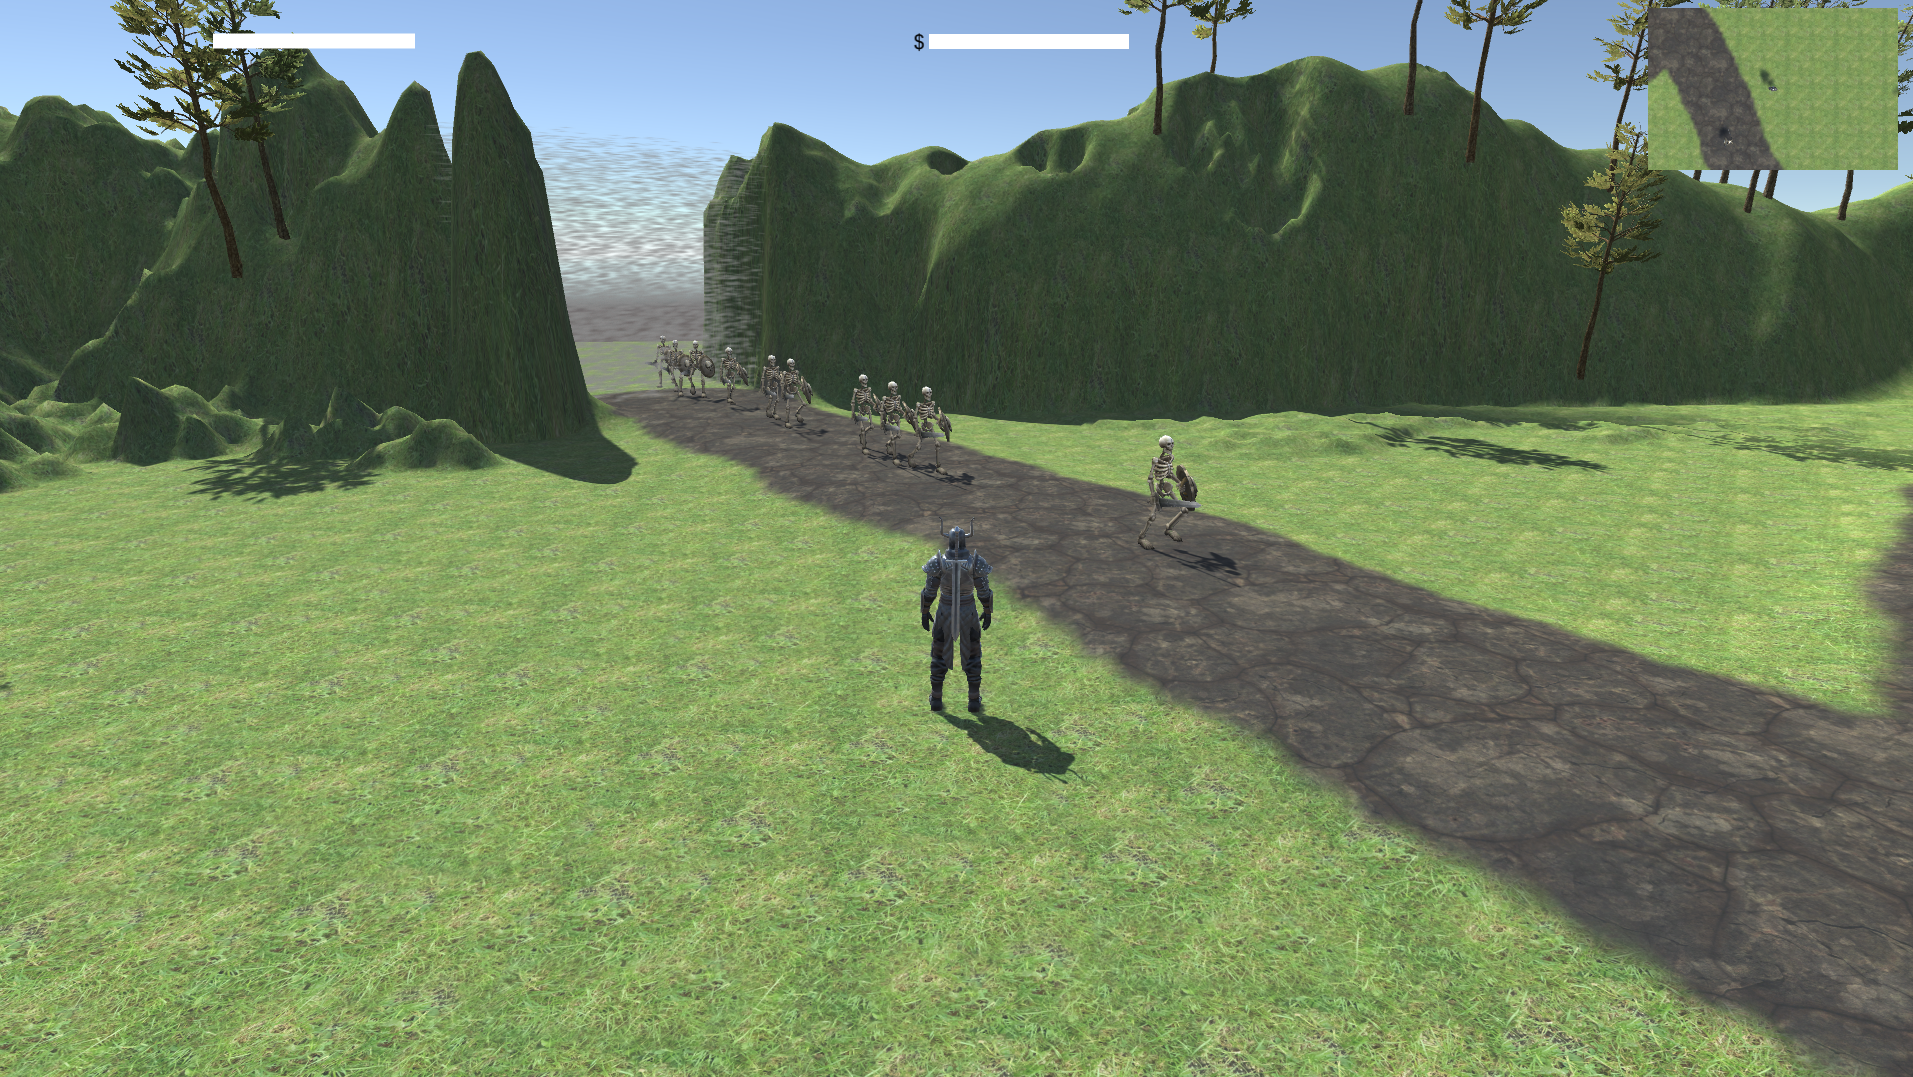
\includegraphics[scale=0.3]{ennemiesprojet.png}}
		\caption*{Apparition d'un vague de squelette}
	\end{figure}

	\subsubsection*{Ce qui est à faire pour la prochaine soutenance}	
	\begin{itemize}
	\item La création d'un inventaire
	\item Un système d'équipement
	\item Ajout de tours et d'autre moyen de d\'efense
	\item Ajout d'un ennemi triant a distance
	\end{itemize}

	\subsection{Animation}
		Les animations permettent de rendre réalistes les mouvements des personnages notamment. Lorsque le héros se déplace, les animations suivent ces mouvements. Elles fonctionnent aussi lorsque le héros court. Une animation lors du saut a également été ajouté. De plus, lorsque le héros inflige des dégâts à ces adversaires, on peut maintenant le voir donner des coups de poing. 
	\par Les ennemis sont également animés. On les voit tous marcher vers le cristal ou bien, vers le héros lorsqu’ils sont dans sa zone de combat.
Il manquera plus que d’animer les ennemis pour rendre leurs attaques fluides. Pour la prochaine soutenance, on essaiera de diversifier les types d’attaque de nos héros. Ainsi, l’overlord pourra sortir une épée et attaquer les monstres avec celle-ci.

\subsubsection*{Ce qui est à faire pour la prochaine soutenance}
\begin{itemize}
\item Animation des personnages
\item Animation des ennemis
\end{itemize}

\section{Planning}
	\begin{tabular}{|c||c|c|c|}
		\hline
		& 1\iere{} soutenance & 2\ieme{} soutenance & 3\ieme{} soutenance \\
		\hline
		Site &  Avancé & Avancé & Terminé \\
		\hline
		3D & Débuté & Avancé & Terminé \\
		\hline
		2D & Débuté & Avancé & Terminé \\
		\hline
		IA & Débuté & Débuté & Terminé\\
		\hline
		Multijoueur & Débuté & Avancé & Terminé\\
		\hline
		Réseau & Débuté & Avancé & Terminé\\
		\hline
		Menu & Avancé & Terminé & Terminé \\
		\hline
		Gameplay & Débuté & Débuté & Terminé\\
		\hline
		Animation & Débuté & Avancé & Terminé\\		
		\hline
		Audio & Non débuté & Débuté & Terminé\\
		\hline		
	\end{tabular}\\
	\newpage
\section{Budget}

Nous sommes des étudiants et ceci est un projet de première année. C'est donc un projet dans le cadre scolaire et à but non lucratif. Ainsi, le budget est de 0\euro{}. Comme prévu aucun achats n'a été nécessaire jusqu'\'a présent pour la réalisation de notre projet. Nous avons utilisé uniquement des logiciels gratuits ou bien fournit gratuitement par l'école. Nous n'avons donc pour le moment aucun dépassement de budget.\\

\centerline{\includegraphics[scale=0.7]{images.jpg}}

\section{Conclusion}

Les outils à notre disposition pour réaliser le projet étant  nouveaux pour nous, nous avons eu du mal à les utiliser de manière efficace. Nous avons dans la mesure du possible essayé de respecter le planning de la première soutenance. Nous avons des l\'eger retards dans la partie multijoueur, mais avons d\'ebut\'e succinctement la partie audio. De nombreuses tâches restent à réaliser pour la deuxième soutenance. Néanmoins, connaissant mieux les outils mis à notre disposition, nous allons travailler beaucoup plus efficacement et nous espérons, respecter le planning pour la deuxième soutenance. 
\end{document}
